\documentclass[]{book}
\usepackage{lmodern}
\usepackage{amssymb,amsmath}
\usepackage{ifxetex,ifluatex}
\usepackage{fixltx2e} % provides \textsubscript
\ifnum 0\ifxetex 1\fi\ifluatex 1\fi=0 % if pdftex
  \usepackage[T1]{fontenc}
  \usepackage[utf8]{inputenc}
\else % if luatex or xelatex
  \ifxetex
    \usepackage{mathspec}
  \else
    \usepackage{fontspec}
  \fi
  \defaultfontfeatures{Ligatures=TeX,Scale=MatchLowercase}
\fi
% use upquote if available, for straight quotes in verbatim environments
\IfFileExists{upquote.sty}{\usepackage{upquote}}{}
% use microtype if available
\IfFileExists{microtype.sty}{%
\usepackage{microtype}
\UseMicrotypeSet[protrusion]{basicmath} % disable protrusion for tt fonts
}{}
\usepackage[margin=1in]{geometry}
\usepackage{hyperref}
\hypersetup{unicode=true,
            pdftitle={Lecture Notes for Biology of Wildlife Populations},
            pdfauthor={Andrew Tyre},
            pdfborder={0 0 0},
            breaklinks=true}
\urlstyle{same}  % don't use monospace font for urls
\usepackage{natbib}
\bibliographystyle{apalike}
\usepackage{color}
\usepackage{fancyvrb}
\newcommand{\VerbBar}{|}
\newcommand{\VERB}{\Verb[commandchars=\\\{\}]}
\DefineVerbatimEnvironment{Highlighting}{Verbatim}{commandchars=\\\{\}}
% Add ',fontsize=\small' for more characters per line
\usepackage{framed}
\definecolor{shadecolor}{RGB}{248,248,248}
\newenvironment{Shaded}{\begin{snugshade}}{\end{snugshade}}
\newcommand{\AlertTok}[1]{\textcolor[rgb]{0.94,0.16,0.16}{#1}}
\newcommand{\AnnotationTok}[1]{\textcolor[rgb]{0.56,0.35,0.01}{\textbf{\textit{#1}}}}
\newcommand{\AttributeTok}[1]{\textcolor[rgb]{0.77,0.63,0.00}{#1}}
\newcommand{\BaseNTok}[1]{\textcolor[rgb]{0.00,0.00,0.81}{#1}}
\newcommand{\BuiltInTok}[1]{#1}
\newcommand{\CharTok}[1]{\textcolor[rgb]{0.31,0.60,0.02}{#1}}
\newcommand{\CommentTok}[1]{\textcolor[rgb]{0.56,0.35,0.01}{\textit{#1}}}
\newcommand{\CommentVarTok}[1]{\textcolor[rgb]{0.56,0.35,0.01}{\textbf{\textit{#1}}}}
\newcommand{\ConstantTok}[1]{\textcolor[rgb]{0.00,0.00,0.00}{#1}}
\newcommand{\ControlFlowTok}[1]{\textcolor[rgb]{0.13,0.29,0.53}{\textbf{#1}}}
\newcommand{\DataTypeTok}[1]{\textcolor[rgb]{0.13,0.29,0.53}{#1}}
\newcommand{\DecValTok}[1]{\textcolor[rgb]{0.00,0.00,0.81}{#1}}
\newcommand{\DocumentationTok}[1]{\textcolor[rgb]{0.56,0.35,0.01}{\textbf{\textit{#1}}}}
\newcommand{\ErrorTok}[1]{\textcolor[rgb]{0.64,0.00,0.00}{\textbf{#1}}}
\newcommand{\ExtensionTok}[1]{#1}
\newcommand{\FloatTok}[1]{\textcolor[rgb]{0.00,0.00,0.81}{#1}}
\newcommand{\FunctionTok}[1]{\textcolor[rgb]{0.00,0.00,0.00}{#1}}
\newcommand{\ImportTok}[1]{#1}
\newcommand{\InformationTok}[1]{\textcolor[rgb]{0.56,0.35,0.01}{\textbf{\textit{#1}}}}
\newcommand{\KeywordTok}[1]{\textcolor[rgb]{0.13,0.29,0.53}{\textbf{#1}}}
\newcommand{\NormalTok}[1]{#1}
\newcommand{\OperatorTok}[1]{\textcolor[rgb]{0.81,0.36,0.00}{\textbf{#1}}}
\newcommand{\OtherTok}[1]{\textcolor[rgb]{0.56,0.35,0.01}{#1}}
\newcommand{\PreprocessorTok}[1]{\textcolor[rgb]{0.56,0.35,0.01}{\textit{#1}}}
\newcommand{\RegionMarkerTok}[1]{#1}
\newcommand{\SpecialCharTok}[1]{\textcolor[rgb]{0.00,0.00,0.00}{#1}}
\newcommand{\SpecialStringTok}[1]{\textcolor[rgb]{0.31,0.60,0.02}{#1}}
\newcommand{\StringTok}[1]{\textcolor[rgb]{0.31,0.60,0.02}{#1}}
\newcommand{\VariableTok}[1]{\textcolor[rgb]{0.00,0.00,0.00}{#1}}
\newcommand{\VerbatimStringTok}[1]{\textcolor[rgb]{0.31,0.60,0.02}{#1}}
\newcommand{\WarningTok}[1]{\textcolor[rgb]{0.56,0.35,0.01}{\textbf{\textit{#1}}}}
\usepackage{longtable,booktabs}
\usepackage{graphicx,grffile}
\makeatletter
\def\maxwidth{\ifdim\Gin@nat@width>\linewidth\linewidth\else\Gin@nat@width\fi}
\def\maxheight{\ifdim\Gin@nat@height>\textheight\textheight\else\Gin@nat@height\fi}
\makeatother
% Scale images if necessary, so that they will not overflow the page
% margins by default, and it is still possible to overwrite the defaults
% using explicit options in \includegraphics[width, height, ...]{}
\setkeys{Gin}{width=\maxwidth,height=\maxheight,keepaspectratio}
\IfFileExists{parskip.sty}{%
\usepackage{parskip}
}{% else
\setlength{\parindent}{0pt}
\setlength{\parskip}{6pt plus 2pt minus 1pt}
}
\setlength{\emergencystretch}{3em}  % prevent overfull lines
\providecommand{\tightlist}{%
  \setlength{\itemsep}{0pt}\setlength{\parskip}{0pt}}
\setcounter{secnumdepth}{5}
% Redefines (sub)paragraphs to behave more like sections
\ifx\paragraph\undefined\else
\let\oldparagraph\paragraph
\renewcommand{\paragraph}[1]{\oldparagraph{#1}\mbox{}}
\fi
\ifx\subparagraph\undefined\else
\let\oldsubparagraph\subparagraph
\renewcommand{\subparagraph}[1]{\oldsubparagraph{#1}\mbox{}}
\fi

%%% Use protect on footnotes to avoid problems with footnotes in titles
\let\rmarkdownfootnote\footnote%
\def\footnote{\protect\rmarkdownfootnote}

%%% Change title format to be more compact
\usepackage{titling}

% Create subtitle command for use in maketitle
\newcommand{\subtitle}[1]{
  \posttitle{
    \begin{center}\large#1\end{center}
    }
}

\setlength{\droptitle}{-2em}

  \title{Lecture Notes for Biology of Wildlife Populations}
    \pretitle{\vspace{\droptitle}\centering\huge}
  \posttitle{\par}
    \author{Andrew Tyre}
    \preauthor{\centering\large\emph}
  \postauthor{\par}
      \predate{\centering\large\emph}
  \postdate{\par}
    \date{2018-12-26}

\usepackage{booktabs}
\newenvironment{rmdnote}
  {}
  {}

\usepackage{amsthm}
\newtheorem{theorem}{Theorem}[chapter]
\newtheorem{lemma}{Lemma}[chapter]
\theoremstyle{definition}
\newtheorem{definition}{Definition}[chapter]
\newtheorem{corollary}{Corollary}[chapter]
\newtheorem{proposition}{Proposition}[chapter]
\theoremstyle{definition}
\newtheorem{example}{Example}[chapter]
\theoremstyle{definition}
\newtheorem{exercise}{Exercise}[chapter]
\theoremstyle{remark}
\newtheorem*{remark}{Remark}
\newtheorem*{solution}{Solution}
\let\BeginKnitrBlock\begin \let\EndKnitrBlock\end
\begin{document}
\maketitle

{
\setcounter{tocdepth}{1}
\tableofcontents
}
\hypertarget{preface}{%
\chapter*{Preface}\label{preface}}
\addcontentsline{toc}{chapter}{Preface}

Placeholder

\hypertarget{chap:fundamental}{%
\chapter{The fundamental law of population
dynamics}\label{chap:fundamental}}

Placeholder

\hypertarget{learning-objectives}{%
\section{Learning objectives}\label{learning-objectives}}

\hypertarget{introduction}{%
\section{Introduction}\label{introduction}}

\hypertarget{killer-whales-and-sea-otters}{%
\subsection{Killer whales and sea
otters}\label{killer-whales-and-sea-otters}}

\hypertarget{the-laws-of-nature}{%
\section{The laws of nature}\label{the-laws-of-nature}}

\hypertarget{the-nature-of-models-of-nature}{%
\section{The nature of models of
nature}\label{the-nature-of-models-of-nature}}

\hypertarget{glossary}{%
\section{Glossary}\label{glossary}}

\hypertarget{chap:sdm}{%
\chapter{Making decisions}\label{chap:sdm}}

Placeholder

\hypertarget{learning-objectives-1}{%
\section{Learning objectives}\label{learning-objectives-1}}

\hypertarget{problem}{%
\section{Problem}\label{problem}}

\hypertarget{objectives}{%
\section{Objectives}\label{objectives}}

\hypertarget{alternatives}{%
\section{Alternatives}\label{alternatives}}

\hypertarget{consequences}{%
\section{Consequences}\label{consequences}}

\hypertarget{tradeoffs}{%
\section{Tradeoffs}\label{tradeoffs}}

\hypertarget{exercises}{%
\section{Exercises}\label{exercises}}

\hypertarget{wild-horses-in-the-american-southwest}{%
\subsection*{Wild horses in the American
Southwest}\label{wild-horses-in-the-american-southwest}}
\addcontentsline{toc}{subsection}{Wild horses in the American Southwest}

\hypertarget{chap:abundance}{%
\chapter{Estimating Abundance}\label{chap:abundance}}

\begin{Shaded}
\begin{Highlighting}[]
\NormalTok{knitr}\OperatorTok{::}\KeywordTok{read_chunk}\NormalTok{(}\StringTok{"R/ci_coverage.r"}\NormalTok{)}
\end{Highlighting}
\end{Shaded}

\hypertarget{learning-objectives-2}{%
\section{Learning objectives}\label{learning-objectives-2}}

At the end of chapter 3, the student should be able to:

General objective: 1. Estimate the abundance of a species within a
specific geographical area, and critically evaluate the utility of
abundance estimates.

Chapter objectives: 1. Estimate population parameters: population size,
density. 2. Estimate the uncertainty of a population estimate in various
ways, and the factors that affect the precision of this uncertainty. 3.
Assess tradeoffs between the accuracy of the information collected and
the objectives proposed in a management scenario.

The fundamental metric of population dynamics is the abundance of the
population. Entire books, indeed lifetimes of research, have been
devoted to this topic. Here I do not attempt a complete coverage of the
topic, but merely introduce the most basic approach -- counting
organisms in a sample of areas of known size. We will learn how to
calculate the uncertainty in an estimate of abundance, and how that
uncertainty changes with effort devoted to sampling. This is an
important concept for a manager of wildlife, because it is necessary to
figure out how much information is good enough for the purpose at hand.
More accurate information is certainly ``better'' in some abstract
sense, but when that accuracy comes at a cost in resources, a tradeoff
(in the very specific sense of chapter \ref{chap:sdm}) must be made
between the accuracy of the information and other objectives to which
those resources could be bent.

Why bother to estimate the size of the population? Why not simply count
every individual animal, and obtain a \emph{census} of the population?
This was standard practice for large mammals in North America until the
middle of the 20\textsuperscript{th} century, and even later in Africa.
With enough well trained personnel, it is indeed possible to obtain high
levels of complete counts for populations, particularly in open areas
like the African savannah. \textbf{The primary reason for abandoning
complete counts is cost.} The time required to survey every piece of a
landscape or region is tremendous, and time is money. In addition, for
many species in many landscapes, the assumption of complete
detectability, that every individual in a sample unit is counted, is not
met. In that case, the attempt to census the population leads to an
abundance that is biased (more on this later). We can both reduce costs
and deal with bias of incomplete detectability by moving to statistical
sampling procedures for estimating the total abundance of a population
in a given area.

The steps required to estimate any parameter in a population, like the
total abundance, follows this general scheme

\begin{Shaded}
\begin{Highlighting}[]
\NormalTok{knitr}\OperatorTok{::}\KeywordTok{include_graphics}\NormalTok{(}\StringTok{"images/Sampling_Design.png"}\NormalTok{)}
\end{Highlighting}
\end{Shaded}

\begin{figure}
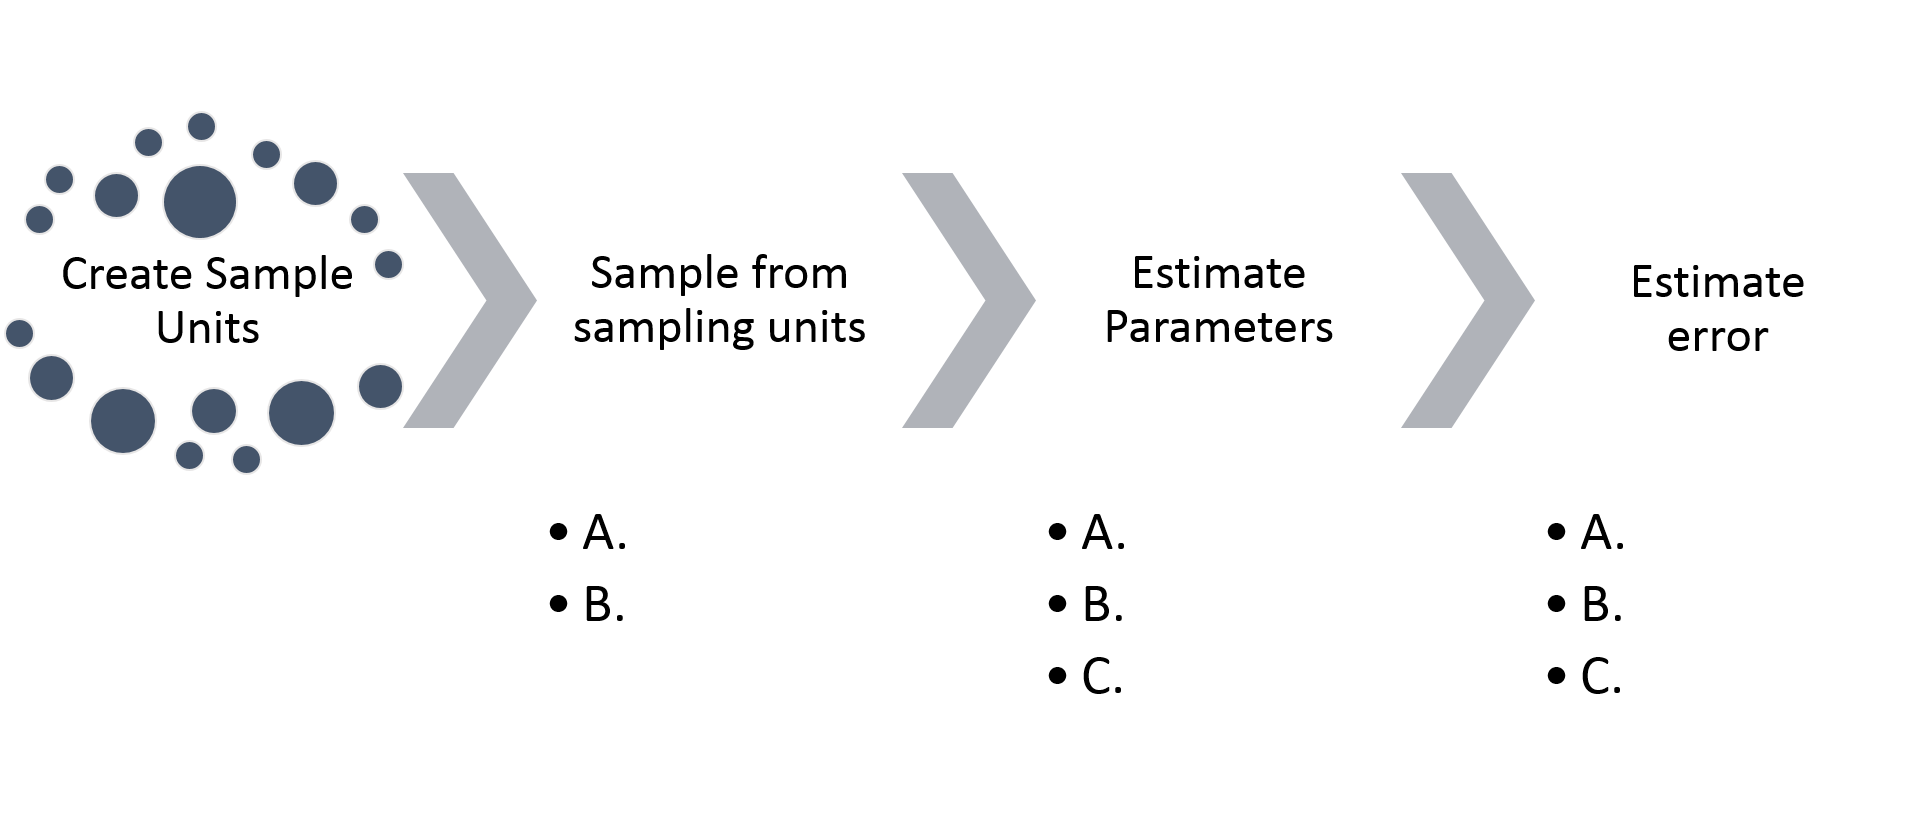
\includegraphics[width=0.49\linewidth]{images/Sampling_Design} \caption{The general steps required to do a simple random sampling.}\label{fig:scheme}
\end{figure}

\hypertarget{sampling-error-accuracy-and-precision}{%
\section{Sampling error, accuracy and
precision}\label{sampling-error-accuracy-and-precision}}

When we want to measure \(N\), the abundance of a population in a
particular area, we have two choices: census or sample. A census means
that every individual is counted -- no one is missed, no one is counted
twice, the answer is \(N\), exactly. In that case, we know what \(N\)
is, and there is no error to estimate. In this case, ``error'' has a
very specific meaning. The error is the difference between the true
\(N\) and the \(N\) that we have measured. In reality, the error is
never zero. Even if a survey of abundance is called a census, it is
virtually impossible to have an exact count of a real population. At
best the error in the count is small and ignorable. A much better
approach is to recognize the existence of error in our counts, and
quantify it. From now on, to distinguish between the true population
abundance, \(N\), and our estimate of the abundance, I will use a
``hat'' to indicate the estimated abundance, like this: \(\hat{N}\).

Error in an estimated quantity like the abundance has two components,
the precision and the accuracy. Precision refers to the variation
between repeated estimates of the same type -- if we sampled the same
population repeatedly, what is the average difference between repeated
samples (Figure \ref{fig:precision})? In contrast, accuracy refers to
the distance between the average estimate and the truth. A good estimate
will on average have no deviation from the true population abundance.
Any individual estimate will be off by some unknown amount, but
averaging repeated samples would converge to the true value. An estimate
of a quantity that has a non-zero average difference between the
estimate and the true value of the quantity is said to be biased. We
want unbiased estimates of abundance.

\begin{Shaded}
\begin{Highlighting}[]
\NormalTok{knitr}\OperatorTok{::}\KeywordTok{include_graphics}\NormalTok{(}\KeywordTok{c}\NormalTok{(}\StringTok{"images/High_precision_Low_accuracy.png"}\NormalTok{, }\StringTok{"images/High_accuracy_Low_precision.png"}\NormalTok{))}
\end{Highlighting}
\end{Shaded}

\begin{figure}
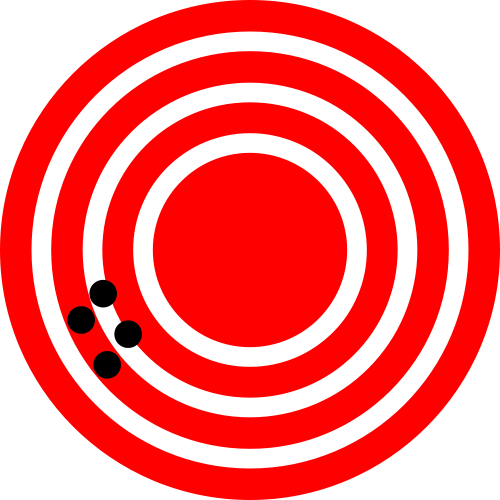
\includegraphics[width=0.49\linewidth]{images/High_precision_Low_accuracy} \includegraphics[width=0.49\linewidth]{images/High_accuracy_Low_precision} \caption{The classic depiction of the difference between accuracy and precision. The figure on the left shows high precision but low accuracy, while the figure on the right shows high accuracy and low precision. (Images from Wikimedia Commons, in the public domain)}\label{fig:precision}
\end{figure}

\hypertarget{simple-random-sampling}{%
\section{Simple random sampling}\label{simple-random-sampling}}

We'll begin with the easiest possible estimate of abundance. We have
some area, \(A\), which we call the \emph{sample frame}. We divide the
sample frame into \(U\) equal sized areas. We'll call these subdivisions
of the area sample units. The area of each sample unit is \(a\), and
\(Ua=A\). We assume that we can count all the individuals in a sample
unit without missing any individuals (perfect detection), and without
counting individuals more than once (no double counting). We cannot
count all \(U\) sample units. If we could, we would have a census, not a
sample. Instead, we will select \(u\) sample units, where typically
\(u\) is much smaller than \(U\). We will select the sample units at
random.

There are two ways to sample randomly from the set of all sample units.
Give each sample unit a unique number, and place strips of paper with
each number into a bag. In the first method, sampling with replacement,
we draw a strip of paper, note the number, and then put the strip of
paper back into the bag. \textbf{This means that it is possible for a
given sample unit to be counted more than once.} In the second method,
sampling without replacement, we draw a strip of paper, note the number,
and then set that strip of paper aside. This means that each sample unit
will only be sampled once. Both methods give the same result for the
estimated abundance, but the precision of the samples will be different,
especially if the total number of sample units U is small. Either way,
we have now obtained a list of sample units in which to count our
individuals.

Having established which units to sample, we now obtain our counts which
I'll label \(y_i\) for the number of individuals counted in sample unit
\(i\). From this dataset I can obtain the point estimate for the
abundance in two steps. First, I calculate the average, or expected
value, of the density for each unit \(\hat{D}\). Second, I multiply this
estimated average by the total area of the sample frame \(A\) to obtain
the estimated abundance. The expected value of \(\hat{D}\) is given by

\begin{equation}
  \hat{D}=\frac{\sum_{i=1}^u{y_i}}{\sum_{i=1}^u{a_i}}
         =\frac{\sum_{i=1}^u{y_i}}{ua}
         =\bar{y}\frac{1}{a}
  \label{eq:densitySWR}
\end{equation}

which has units of individuals per unit area. If you look back into your
introductory statistics textbook, this is simply the arithmetic mean
(\(\bar{y}\)) multiplied by \(1/a\). This is the conversion from an
average count per sample unit to an average density per unit area. The
estimated abundance in the entire area is then

\begin{equation}
  \hat{N}=\hat{D}A.
  \label{eq:abundance}
\end{equation}

\textbf{This estimate will be unbiased, or accurate, if our counts in
each sample unit are made without errors. All individuals present are
detected, no individuals are counted twice, and no other species are
mistakenly identified as the species of interest.} These are challenging
conditions to meet, in most cases.

The next step is to quantify the precision of our estimate. This is the
step that differs between sampling with and without replacement. The
simplest formula is for the case where sampling is done with
replacement. This is the same formula for the standard error of a mean
when sampling from an infinite population. The first step is to
calculate the sample variance of the counts

\[
s_y^2 = \frac{\sum_{i=1}^{u}{y_i^2}-\frac{\left(\sum_{i=1}^u{y_i}\right)^2}{u}}
               {u-1}
  \label{eq:samplevariance}
\]

This is the variance of the distribution of the counts, not yet the
precision of our sample mean. The sample variance is a property of the
observed counts. In contrast, the precision of our sample mean is a
property of a statistic, the average density. This statistic itself has
a distribution, that is, it is a random variable whose value is not
known precisely. Imagine taking a second, and then a third, sample of
units and recalculating the average density. Each time you take a
sample, the average density will be different. Imagine doing that
infinitely many times, and you have the distribution of the average
density.

The best estimate of the expected value of the distribution of the
average density is just the sample mean. But what about the variance of
the distribution of the average density? The sample variance seems
relevant; a more variable sample should lead to a less precise estimate
of the sample mean. Intuitively, as more data are collected, the
precision should improve the estimate of the mean gets better. So the
variance of our average density should increase with the sample variance
and decrease with the sample size, and it turns out that

\begin{equation}
  s_{\hat{D}}^2 = \frac{1}{a^2}\frac{s_y^2}{u}
  \label{eq:densityvarwr}
\end{equation}

is an unbiased estimate of the variance of the density. The square root
of this variance \(s_{\hat{D}}\) is given a special name, the standard
error of the density. The term with \(a^2\) in the denominator simply
ensures that the correct units are maintained.

What if the sample was taken without replacement? In this case the
finiteness of the sample has to be taken into account. As the number of
samples taken, \(u\), increases towards the number of sample units
available the sample becomes less of a sample and more of a census. In
the extreme, sampling all of the units, the count is a census with no
sampling variation at all. Thus the precision of our estimated mean
should increase as the fraction of sample units counted increases.
Equivalently, this means that the variance of the sample mean should
decrease as the number of units counted rises towards the number
available. The usual way to achieve this is to use the \emph{finite
population correction} in the formula for the variance of the sample
mean

\begin{equation}
  s_{\hat{D}}^2 = \frac{1}{a^2}\frac{s_y^2}{u}\left(1-\frac{u}{U}\right)
  \label{eq:densityvarwor}
\end{equation}

And when \(u = U\) this extra term equals zero, and the variance of the
sample mean is zero. As a result of this correction factor, estimates
from a sample without replacement are always more precise than a sample
taken with replacement.

The last step is to estimate the precision of the abundance \(\hat{N}\).
This quantity is a function of a random variable, \(\hat{D}\), and a
constant \(A\). There are several different ways to justify this, but
for now just accept that the variance of the product of a random
variable and a constant is just the product of the variance and the
constant squared. In words that doesn't sound so good, so here it is as
a formula:

\begin{equation}
  s_{\hat{N}}^2= s_{\hat{D}}^2 A^2
  \label{eq:abundancevar}
\end{equation}

which is pretty easy.

With the estimated abundance and it's precision in hand, there are a
couple of other numbers worth calculating. The coefficient of variation
is simply

\begin{equation}
  CV_{\hat{N}} =\frac{s_{\hat{N}}}{\hat{N}}  100
  \label{eq:cv}
\end{equation}

or the ratio between the standard error of abundance and abundance
multiplied by 100. The CV is a useful relative measure of precision that
can be readily compared between different estimates. Imagine you have 2
estimates, one of 100 individuals with a standard error of 10 and the
second of a 1000 individuals with a standard error of 50. Which estimate
is more precise? In an absolute sense the first estimate has a smaller
standard error. However, in a relative sense, the second one is more
precise with a CV of 5\% compared to a CV of 10\%. Implicit in the use
of the CV is that a deviation of a given size is less important if the
abundance is larger.

When presenting estimated abundances graphically or in tables it is
standard practice to convert the estimates of the precision into
confidence limits on the estimate. A confidence limit shows the range of
values that would contain the true mean a certain percentage of the
time, typically 95\%, if the entire estimation process (including
calculating the confidence limits) were repeated many times (Figure
\ref{fig:ciCoverage}). This is a challenging concept to grasp ---
however there are a couple of simple rules for interpreting these
limits. First, you may not infer that the distribution of possible
population sizes is indicated by the confidence limits. Unfortunately
this is exactly what most biologists would like to do. Second, smaller
confidence intervals are better. Third, \textbf{if the confidence limits
do not include some specific constant (like a target population size),
then you can say that the estimate is statistically significantly
different from the constant value.}

\begin{Shaded}
\begin{Highlighting}[]
\CommentTok{# abundance CI coverage}
\CommentTok{# }
\NormalTok{U =}\StringTok{ }\DecValTok{100}
\NormalTok{u =}\StringTok{ }\DecValTok{10}
\NormalTok{N =}\StringTok{ }\DecValTok{100}
\NormalTok{n.true=}\KeywordTok{rnorm}\NormalTok{(U,N}\OperatorTok{/}\NormalTok{U)}
\CommentTok{#sum(n.true)}
\CommentTok{# sampling with replacement}
\NormalTok{sample.it <-}\StringTok{ }\ControlFlowTok{function}\NormalTok{(x,n,U,u)\{}
\NormalTok{  n =}\StringTok{ }\KeywordTok{sample}\NormalTok{(n,u,}\DataTypeTok{replace=}\OtherTok{TRUE}\NormalTok{)}
\NormalTok{  somevariable =}\StringTok{ }\NormalTok{x}
\NormalTok{  N.hat =}\StringTok{ }\KeywordTok{mean}\NormalTok{(n)}\OperatorTok{*}\NormalTok{U}
\NormalTok{  N.var =}\StringTok{ }\NormalTok{U}\OperatorTok{^}\DecValTok{2}\OperatorTok{*}\KeywordTok{var}\NormalTok{(n)}\OperatorTok{/}\NormalTok{u}
\NormalTok{  N.CI =}\StringTok{ }\KeywordTok{c}\NormalTok{(N.hat}\OperatorTok{-}\KeywordTok{qt}\NormalTok{(}\FloatTok{0.975}\NormalTok{,}\DecValTok{9}\NormalTok{)}\OperatorTok{*}\KeywordTok{sqrt}\NormalTok{(N.var),N.hat}\OperatorTok{+}\KeywordTok{qt}\NormalTok{(}\FloatTok{0.975}\NormalTok{,}\DecValTok{9}\NormalTok{)}\OperatorTok{*}\KeywordTok{sqrt}\NormalTok{(N.var))}
  \KeywordTok{return}\NormalTok{(}\KeywordTok{c}\NormalTok{(N.hat,N.var,N.CI))}
\NormalTok{\}}

\NormalTok{samples =}\StringTok{ }\KeywordTok{sapply}\NormalTok{(}\DecValTok{1}\OperatorTok{:}\DecValTok{20}\NormalTok{,sample.it,}\DataTypeTok{U=}\NormalTok{U,}\DataTypeTok{u=}\NormalTok{u,}\DataTypeTok{n=}\NormalTok{n.true)}
\KeywordTok{plot}\NormalTok{(samples[}\DecValTok{1}\NormalTok{,],}\DataTypeTok{ylim=}\KeywordTok{range}\NormalTok{(samples[}\DecValTok{3}\OperatorTok{:}\DecValTok{4}\NormalTok{,]),}\DataTypeTok{pch=}\DecValTok{19}\NormalTok{,}\DataTypeTok{axes=}\OtherTok{FALSE}\NormalTok{,}\DataTypeTok{xlab=}\StringTok{""}\NormalTok{,}\DataTypeTok{ylab=}\StringTok{"Abundance"}\NormalTok{)}
\KeywordTok{box}\NormalTok{()}
\KeywordTok{axis}\NormalTok{(}\DecValTok{2}\NormalTok{,}\DataTypeTok{at=}\KeywordTok{seq}\NormalTok{(}\DecValTok{0}\NormalTok{,}\DecValTok{200}\NormalTok{,}\DecValTok{50}\NormalTok{))}
\KeywordTok{arrows}\NormalTok{(}\DecValTok{1}\OperatorTok{:}\DecValTok{20}\NormalTok{,samples[}\DecValTok{3}\NormalTok{,],}\DecValTok{1}\OperatorTok{:}\DecValTok{20}\NormalTok{,samples[}\DecValTok{4}\NormalTok{,],}\DataTypeTok{angle=}\DecValTok{90}\NormalTok{,}\DataTypeTok{code=}\DecValTok{3}\NormalTok{,}\DataTypeTok{length=}\FloatTok{0.1}\NormalTok{)}
\KeywordTok{abline}\NormalTok{(}\DataTypeTok{h=}\KeywordTok{sum}\NormalTok{(n.true),}\DataTypeTok{lty=}\DecValTok{2}\NormalTok{)}
\end{Highlighting}
\end{Shaded}

\begin{figure}
\centering
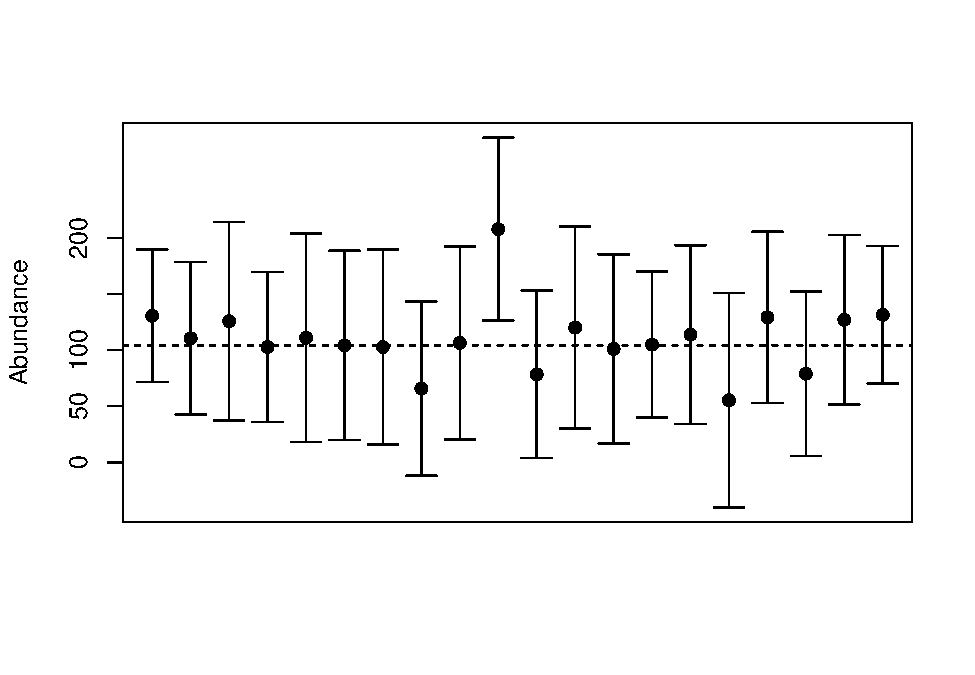
\includegraphics{NRES450-LectureNotes_files/figure-latex/ciCoverage-1.pdf}
\caption{\label{fig:ciCoverage}Simulated abundance estimates with 95\%
confidence intervals. The horizontal dashed line is the true abundance
in a sample frame with 100 units. The dots represent 20 different
samples of 10 units (with replacement) from the sample frame.}
\end{figure}

\hypertarget{how-big-a-sample-to-take}{%
\section{How big a sample to take?}\label{how-big-a-sample-to-take}}

\begin{Shaded}
\begin{Highlighting}[]
\NormalTok{u <-}\StringTok{ }\DecValTok{2}\OperatorTok{:}\DecValTok{100}
\NormalTok{var <-}\StringTok{ }\NormalTok{D <-}\StringTok{ }\DecValTok{10}
\NormalTok{SE <-}\StringTok{ }\KeywordTok{sqrt}\NormalTok{(var}\OperatorTok{/}\NormalTok{u)}
\NormalTok{CV <-}\StringTok{ }\NormalTok{SE}\OperatorTok{/}\NormalTok{D}
\KeywordTok{plot}\NormalTok{(SE}\OperatorTok{~}\NormalTok{u,}\DataTypeTok{xlab=}\StringTok{"Sample size"}\NormalTok{,}\DataTypeTok{ylab=}\StringTok{"Standard Error"}\NormalTok{,}\DataTypeTok{type=}\StringTok{"l"}\NormalTok{,}\DataTypeTok{lwd=}\DecValTok{3}\NormalTok{)}
\KeywordTok{box}\NormalTok{()}
\NormalTok{D <-}\StringTok{ }\DecValTok{10}
\NormalTok{var <-}\StringTok{ }\DecValTok{20}
\NormalTok{SE <-}\StringTok{ }\KeywordTok{sqrt}\NormalTok{(var}\OperatorTok{/}\NormalTok{u)}
\NormalTok{CV <-}\StringTok{ }\NormalTok{SE}\OperatorTok{/}\NormalTok{D}
\KeywordTok{lines}\NormalTok{(SE}\OperatorTok{~}\NormalTok{u,}\DataTypeTok{col=}\StringTok{"red"}\NormalTok{)}
\NormalTok{D <-}\StringTok{ }\DecValTok{10}
\NormalTok{var <-}\StringTok{ }\DecValTok{5}
\NormalTok{SE <-}\StringTok{ }\KeywordTok{sqrt}\NormalTok{(var}\OperatorTok{/}\NormalTok{u)}
\NormalTok{CV <-}\StringTok{ }\NormalTok{SE}\OperatorTok{/}\NormalTok{D}
\KeywordTok{lines}\NormalTok{(SE}\OperatorTok{~}\NormalTok{u,}\DataTypeTok{col=}\StringTok{"green"}\NormalTok{)}
\end{Highlighting}
\end{Shaded}

\begin{figure}
\centering
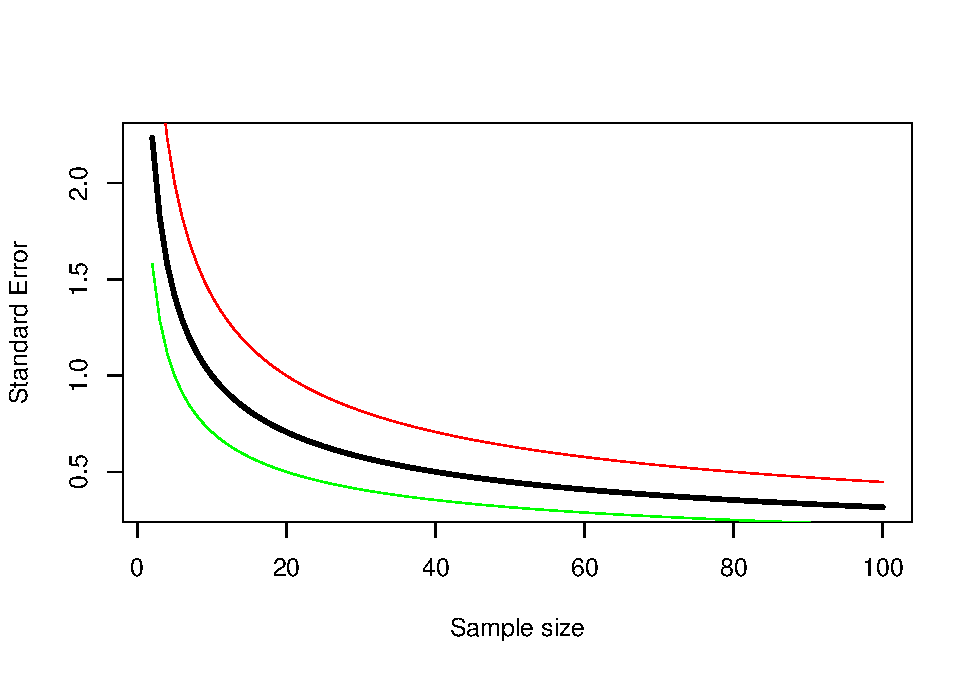
\includegraphics{NRES450-LectureNotes_files/figure-latex/sampleSize-1.pdf}
\caption{\label{fig:sampleSize}The standard error decreases as sample size
increases. This assumes simple random sampling with replacement, and
each count has a mean of 10 and a variance of 5 (green line), 10 (black
line), or 20 (red line).}
\end{figure}

Should we care how many units we sample? Each additional unit increases
the cost of the effort - at a minimum it takes time, and time is usually
money. So why not use the smallest number of units possible? We can
calculate a variance with a sample size of two, so why not use only two?

As always in life, there is a tradeoff to be made here. Fewer sample
units are cheaper, but the resulting estimate is less precise.
Unfortunately, there is no ``rule of thumb'' that works for all samples.
The greater the sample size, the more precise the estimate is all one
can say. The response is also not linear -- when sample sizes are small
the increase in precision with each additional sample is greater than
when sample sizes are large (Figure \ref{fig:sampleSize}). The exact
height of this curve depends on the variance of the counts in each
sample unit, but the shape of the curve will always be a reciprocal
function of the sample size. The curve is higher (worse precision for a
given sample size) when the variance of the counts is higher for the
same average count (red line in Figure \ref{fig:sampleSize}). The curve
is lower (better precision for a given sample size) when the variance is
smaller (green line in Figure \ref{fig:sampleSize}).

So how do we decide on the number of samples to take? We need to have
some information about the mean and variance of the samples we are going
to take, and a goal for the precision of our estimate. There are rules
of thumb for the precision required, but they are nearly impossible to
achieve. For rough monitoring a coefficient of variation of 20\% is
considered acceptable, while for research purposes 5\% is the goal. The
expected mean and variance of the samples comes either from previous
surveys of the same species using the same methods, or expert opinion
(also known as a SWAG for Scientific Wild Assed Guess). With this
information it is possible to construct the curve in Figure
\ref{fig:sampleSize}, and then read off the sample size needed to
achieve the goal. What typically happens is that the budget available
sets the precision that can be achieved.

It is important to note that the variance of the counts is \emph{not} a
function of the sample size. The estimated sample variance will change
as more samples are taken, but does not change systematically. Rather,
the sample variance converges towards the true variance of the counts,
which is some positive number (Figure \ref{fig:samplevar}). At small
sample sizes the variance of the sample variance is also higher.

\begin{Shaded}
\begin{Highlighting}[]
\NormalTok{u <-}\StringTok{ }\DecValTok{2}\OperatorTok{:}\DecValTok{100}
\NormalTok{var <-}\StringTok{ }\NormalTok{D <-}\StringTok{ }\DecValTok{10}
\NormalTok{Y =}\StringTok{ }\KeywordTok{sapply}\NormalTok{(u,}\ControlFlowTok{function}\NormalTok{(x)}\KeywordTok{rnorm}\NormalTok{(x,D,}\KeywordTok{sqrt}\NormalTok{(var)))}
\NormalTok{v =}\StringTok{ }\KeywordTok{sapply}\NormalTok{(Y,var)}
\KeywordTok{plot}\NormalTok{(v}\OperatorTok{~}\NormalTok{u,}\DataTypeTok{xlab=}\StringTok{"Sample Size"}\NormalTok{,}\DataTypeTok{ylab=}\StringTok{"Sample variance"}\NormalTok{,}\DataTypeTok{pch=}\DecValTok{19}\NormalTok{)}
\KeywordTok{abline}\NormalTok{(}\DataTypeTok{h=}\NormalTok{var,}\DataTypeTok{lty=}\DecValTok{2}\NormalTok{)}
\end{Highlighting}
\end{Shaded}

\begin{figure}
\centering
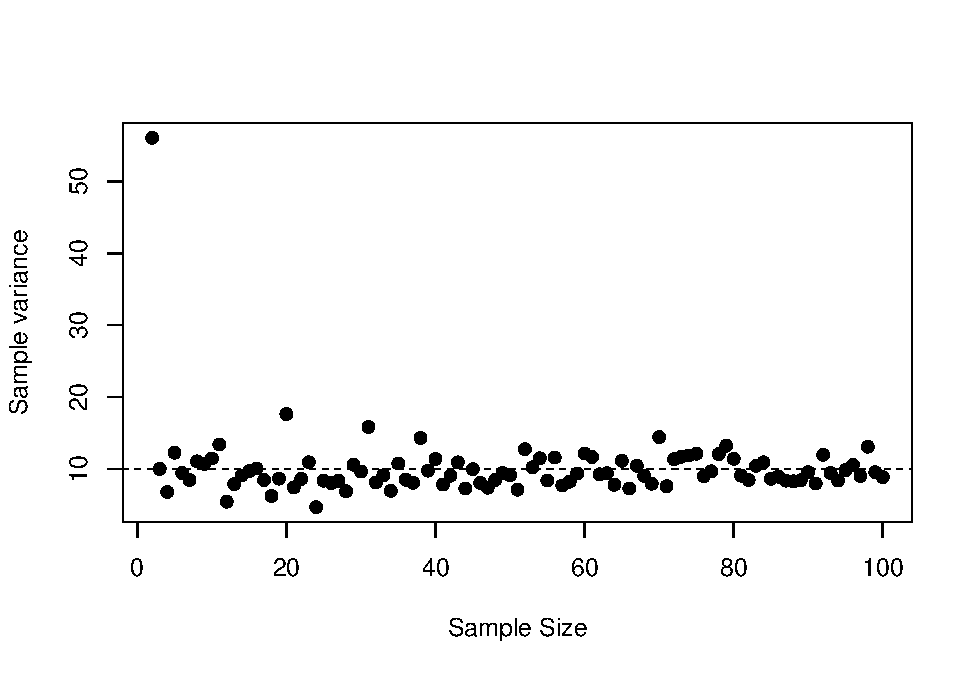
\includegraphics{NRES450-LectureNotes_files/figure-latex/samplevar-1.pdf}
\caption{\label{fig:samplevar}The variance of the counts does not
systematically decrease as the sample size increases. The dashed line is
the true variance for each sample}
\end{figure}

\hypertarget{areas-of-different-sizes}{%
\section{Areas of different sizes}\label{areas-of-different-sizes}}

In the previous section the sample units were equal in size, so that the
total area \(A = Ua\). In many instances the sample units may not be
equal in size, and then a slightly different approach is needed for
calculating the precision of the total abundance \(N\). The first issue
is to choose the sample units randomly with respect to their size. The
second issue is how to deal with differences in size when calculating
the standard errors of density and hence abundance.

One option for choosing sample units that differ in size is to ignore
the differences, and choose sample units with equal probabilities. This
leads to a \emph{ratio estimate} of the abundance. The estimate of the
density is

\begin{equation}
  \hat{D} =  \frac{\sum_{i=1}^u{y_i}}{\sum_{i=1}^u{a_i}}
  \label{eq:densityRatio}
\end{equation}

which leads to an abundance estimate given by

\begin{equation}
  \hat{N} = \hat{D} A.
\end{equation}

This is identical to the estimator used when the sample units have
identical areas. The formula for the sample variance of the \(y_i\) is
different because each count is weighted in the variance differently.

\begin{equation}
  s_y^2 = \frac{\sum_{i=1}^u{y_i^2}+\hat{D}^2\sum_{i=1}^u{a_i^2}-2\hat{D}\sum_{i=1}^u{a_iy_i}}{\left(u-1\right)}.
  \label{eq:samplevarianceRatio}
\end{equation}

With the sample variance for the counts calculated, we follow the same
procedure to get the the variance of \(\hat{D}\)

\begin{equation}
  s_{\hat{D}}^2 = \left(\frac{u}{\sum_{i=1}^u{a_i}}\right)^2\frac{s_y^2}{u}
  \label{eq:densityvarwrRatio}
\end{equation}

The finite sample size correction for sampling without replacement is
similar - now instead of the fraction of sample units we use the
fraction of the area:

\begin{equation}
  s_{\hat{D},SWOR}^2 = s_{\hat{D}}^2\left(1-\frac{\sum_{i=1}^u{a_i}}{A}\right).
  \label{eq:densityvarworRatio}
\end{equation}

Finally, the conversion to the \(s_{\hat{N}}^2\) is always the same,
simply multiplying the variance by the square of total area, \(A\).

\[
  s_{\hat{N}}^2 = s_{\hat{D}}^2 A^2 
\]

The second alternative is to select sample units with a probability
proportional to their size; this leads to a
\emph{probability-proportional-to-size} or PPS estimate. For example, if
our sample units are defined in a GIS layer with different size
polygons, and we select the units to be sampled by throwing random
points onto the map, then each unit will be selected with a probability
proportional to it's size. In addition, it will also be sampling with
replacement, and this is the only type of sampling that works for this
estimator.

\hypertarget{stratified-sampling}{%
\section{Stratified Sampling}\label{stratified-sampling}}

So far, all sampling has been carried out as simple random sampling,
either with or without replacement. It turns out that this may not give
the most accurate estimate of abundance. The implicit assumption is that
all sample units have the same statistical parameters, that is, the same
mean and variance of counts. If this is not true, if there are
differences between sample units, then simple random sampling does not
yield the most accurate estimate of abundance.

How might such differences arise? The most obvious differences are
ecological - not all areas are equally good habitat for a species. We
expect to find more individuals in areas that are better habitat, and
all else being equal, more individuals also means an increase in the
variance of our counts. This kind of heterogeneity is the rule, rather
than the exception, and therefore our simple random sampling is usually
not the best estimator.

In the presence of heterogeneity, the best estimate of abundance
requires \emph{stratified random sampling}, where \textbf{the
probability of selecting a sample unit is made proportional to the
variance of the counts in that unit.} In this way, more data are
collected where the variances are greater, and the resulting estimate is
more accurate. You might already be able to see the catch - how do we
know which units have greater variance before we collect any data? As
always, nothing comes for free!

If we know what the variances are, then everything is easy. The sample
frame is divided into strata in such a way that the variances in counts
are equal within strata (or at least more equal within than between
strata). There is a tradeoff to be made here -- more strata means the
heterogeneity within a stratum is smaller, but eventually the added
complexity becomes self defeating. Strata that are larger or have higher
variance receive a larger proportion of the sample units

\begin{equation}
  u_h = u \frac{U_{h} SE\left(\hat{N_h}\right)}
               {\sum_{i=1}^{H}{U_{h} SE\left(\hat{N_h}\right)}}
  \label{eq:neymanallocation}
\end{equation}

where \(u\) is the total sampling effort to be allocated, and \(U_h\) is
the total number of sample units available in stratum \(h\). This
allocation, known as the Neyman allocation, is optimal, in the sense
that the variance of \(\hat{N}\) is as small as possible. If the cost of
sampling each stratum is identical, then this will also yield the most
precise estimate for a given cost. However, if sampling costs differ
between strata, then we also want to change the proportion with the cost
of each stratum in order to do the best possible for a given amount of
money.

What if we don't know what the variances are? Typically we still have
some notion of where we expect to find more or less of the species in
question. Ideally, we already have the landscape categorized in some
fashion, say into ecoregions, and we know that some ecoregional types
are better than others. Or we know that certain land uses are more
conducive to the species. For example, if you want to estimate the
abundance of a prairie dependent species like the grasshopper sparrow,
you would expect fewer of them in riparian forests than in perennial
grasslands. In addition, the variance of a count typically increases
with the abundance (see \protect\hyperlink{taylors-law}{Taylor's Law}).
Thus for stratification to work, it is sufficient to have an idea of the
relative abundance, and hence relative variance in counts.

Once we've divided the sample frame into \(H\) strata and decided how
many units to sample in each stratum, we then simply calculate the
abundance for each stratum \(h\) using the formulas given previously,
and add them together

\begin{equation}
   \hat{N} = \sum_{i=1}^{H}{\hat{N_h}}.
   \label{eq:abundanceStratified}
\end{equation}

The \(\hat{N_h}\) for each stratum are calculated in exactly the same
way as the abundance estimates for simple random sampling. Similarly, we
can get the variance of the abundance as the sum of the variances of
each stratum estimate.

\begin{equation}
   var\left(\hat{N}\right) = \sum_{i=1}^{H}{var\left(\hat{N_h}\right)}.
   \label{eq:abundancevarianceStratfied}
\end{equation}

Imagine that you want to estimate the population of white tailed deer
(\emph{Odocoileus virginianus}) on a property along the Platte River in
Nebraska. The property has two kind of habitats, riparian forest and
upland pasture. You know that deer prefer forests, and so you expect
deer to be four times as abundant in the forest as they are in the
pasture. You're planning drive counts on 10 ha blocks, and there are 100
ha of each type of habitat, so \(U_{forest} = U_{pasture} = 10\). If we
can afford to carry out \(u_{total} = 6\) drive counts, how many should
we do in the forest vs.~the pasture?

\begin{equation}
  u_{forest} = u_{total} \frac{U_{forest} SE_{forest}}
               {U_{forest} SE_{forest} + U_{pasture} SE_{pasture}} \
           = 6 \frac{10\cdot \sqrt{4}}
                  {10 \cdot \sqrt{4} + 10 \cdot \sqrt{1}} \
           = 6 \frac{20}
                  {20 + 10} \
           = 4
\end{equation}

In that case we should do 4 counts in the forest and 2 in the pasture.
Note that we use the square root of the relative abundances, because the
variance is proportional to abundance, but the allocation equation uses
the standard errors. Even though the relative areas of the two habitats
are identical, we do more counts in the forest because we expect the
variance of the counts to be higher there.

\BeginKnitrBlock{rmdnote}
\hypertarget{taylors-law}{%
\subsection*{Taylor's Law}\label{taylors-law}}
\addcontentsline{toc}{subsection}{Taylor's Law}

One of the most repeatable patterns in ecology is the relationship
between the mean abundance and the variance of sample counts Ecologist
Richard Southwood named this relationship ``Taylor's law'' after his
colleague L.R. Taylor, although it was known from agricultural data long
before Taylor presented it in a 1961 Nature paper. In it's linear form
Taylor's law is

\[
  log\left(s_y^2\right) = a + b \cdot log\left(D\right)\,.
\]

It is possible to use simple linear regression to estimate the constants
\(a\) and \(b\) if you have estimates of the density from areas with a
range of densities. The constant \(b\) can be shown to be equal to 1
when the organisms are distributed at random. Values of \(b\) less than
one are indications of underdispersion, or even spacing between
individuals, while values of \(b > 1\) indicate aggregation between
individuals. Thus, \textbf{if the variance of the counts is greater than
the mean of the counts, we say the population is ``overdispersed''}, or
equivalently, that individuals are clumped together more than we expect
from a random distribution.
\EndKnitrBlock{rmdnote}

\hypertarget{further-reading}{%
\section*{Further Reading}\label{further-reading}}
\addcontentsline{toc}{section}{Further Reading}

Thompson, William, \emph{et al.}(1998) Monitoring Vertebrate
Populations. Academic Press.

There's a good cheat sheet for sample means and variances at
\url{''http://www.uky.edu/~jmlhot2/courses/for480/Forest\%20Sampling\%20Forumla\%20Sheet.pdf''}

\hypertarget{exercises-1}{%
\section*{Exercises}\label{exercises-1}}
\addcontentsline{toc}{section}{Exercises}

\begin{Shaded}
\begin{Highlighting}[]
\KeywordTok{options}\NormalTok{(}\DataTypeTok{knitr.kable.NA =} \StringTok{''}\NormalTok{)}
\NormalTok{caribou <-}\StringTok{ }\NormalTok{readr}\OperatorTok{::}\KeywordTok{read_delim}\NormalTok{(}
\StringTok{"Stratum & Stratum Size, $U_h$ & Sample Size, $u_h$ & Mean # caribou per sample unit & Variance of counts  $S_y^2$ & $N_h$ & $var(N_h)$}
\StringTok{A & 400 & 98  & 24.1 & 5575 &       &     }
\StringTok{B & 30  & 10  & 25.6 & 4064 & NA  & NA }
\StringTok{C & 61  & 37  & 267.6 & 347556 & NA  &  NA}
\StringTok{D & 18  & 6   & 179 & 22798 & NA & NA}
\StringTok{E & 70  & 39  & 293.7 & 123578 & NA  & NA}
\StringTok{F & 120 & 21  & 33.2 & 9795 & NA &  NA}
\StringTok{Total & 699 & 211 & NA & NA & NA & NA "}\NormalTok{, }\DataTypeTok{delim=}\StringTok{"&"}\NormalTok{, }\DataTypeTok{col_names=}\OtherTok{TRUE}\NormalTok{)}
\NormalTok{knitr}\OperatorTok{::}\KeywordTok{kable}\NormalTok{(caribou, }\DataTypeTok{caption=}\StringTok{"Stratified random sample of the Nelchina Caribou herd in Alaska by Sniff and Skoog (1964). Units are 4 square miles."}\NormalTok{)}
\end{Highlighting}
\end{Shaded}

\begin{table}

\caption{\label{tab:caribouExample}Stratified random sample of the Nelchina Caribou herd in Alaska by Sniff and Skoog (1964). Units are 4 square miles.}
\centering
\begin{tabular}[t]{l|l|l|l|l|l|l}
\hline
Stratum  &  Stratum Size, \$U\_h\$  &  Sample Size, \$u\_h\$  &  Mean \# caribou per sample unit  &  Variance of counts  \$S\_y\textasciicircum{}2\$  &  \$N\_h\$  &  \$var(N\_h)\$\\
\hline
A & 400 & 98 & 24.1 & 5575 &  & \\
\hline
B & 30 & 10 & 25.6 & 4064 & NA & NA\\
\hline
C & 61 & 37 & 267.6 & 347556 & NA & NA\\
\hline
D & 18 & 6 & 179 & 22798 & NA & NA\\
\hline
E & 70 & 39 & 293.7 & 123578 & NA & NA\\
\hline
F & 120 & 21 & 33.2 & 9795 & NA & NA\\
\hline
Total & 699 & 211 & NA & NA & NA & NA\\
\hline
\end{tabular}
\end{table}

\begin{enumerate}
\def\labelenumi{\arabic{enumi}.}
\item
  Calculate the estimated abundance and variance of the entire Nelchina
  Caribou Herd (Table \ref{tab:caribouExample}).
\item
  Given the same total sample size, what is the Neyman allocation of
  sample units to strata in the Caribou example?
\end{enumerate}

\hypertarget{chap:exponential}{%
\chapter{Exponential growth and decay}\label{chap:exponential}}

Placeholder

\hypertarget{deaths}{%
\section{Deaths}\label{deaths}}

\hypertarget{births}{%
\section{Births}\label{births}}

\hypertarget{turchins-law-of-population-inertia}{%
\section{Turchin's law of population
inertia}\label{turchins-law-of-population-inertia}}

\hypertarget{estimating-r}{%
\section{\texorpdfstring{Estimating
\(r\)}{Estimating r}}\label{estimating-r}}

\hypertarget{glossary-1}{%
\section{Glossary}\label{glossary-1}}

\hypertarget{exercises-2}{%
\section{Exercises}\label{exercises-2}}

\hypertarget{chap:regulation}{%
\chapter{Population Regulation and
Stochasticity}\label{chap:regulation}}

Placeholder

\hypertarget{pheasants-on-the-island}{%
\subsection*{Pheasants on the Island}\label{pheasants-on-the-island}}
\addcontentsline{toc}{subsection}{Pheasants on the Island}

\hypertarget{resource-limitation}{%
\section{Resource Limitation}\label{resource-limitation}}

\hypertarget{the-many-flavors-of-carrying-capacity}{%
\subsection{The many flavors of carrying
capacity}\label{the-many-flavors-of-carrying-capacity}}

\hypertarget{density-dependent-or-independent}{%
\section{Density Dependent or
Independent?}\label{density-dependent-or-independent}}

\hypertarget{stochasticity}{%
\section{Stochasticity}\label{stochasticity}}

\hypertarget{trends-over-time}{%
\section{Trends over time}\label{trends-over-time}}

\hypertarget{glossary-2}{%
\section{Glossary}\label{glossary-2}}

\hypertarget{chap:harvesting}{%
\chapter{Harvesting and Control}\label{chap:harvesting}}

Placeholder

\hypertarget{eurasian-lynx-in-norway}{%
\subsection*{Eurasian Lynx in Norway}\label{eurasian-lynx-in-norway}}
\addcontentsline{toc}{subsection}{Eurasian Lynx in Norway}

\hypertarget{standard-model}{%
\section{Compensatory and Additive Mortality}\label{standard-model}}

\hypertarget{better-model}{%
\section{A Better Model For Harvesting Wildlife}\label{better-model}}

\hypertarget{epitaph-for-msy}{%
\subsection*{Epitaph for MSY}\label{epitaph-for-msy}}
\addcontentsline{toc}{subsection}{Epitaph for MSY}

\hypertarget{fixed-quota-harvesting}{%
\subsection{Fixed quota harvesting}\label{fixed-quota-harvesting}}

\hypertarget{fixed-effort-harvest-strategy}{%
\subsection{Fixed Effort harvest
strategy}\label{fixed-effort-harvest-strategy}}

\hypertarget{revisiting-eurasian-lynx}{%
\subsection{Revisiting Eurasian Lynx}\label{revisiting-eurasian-lynx}}

\hypertarget{revisiting-additivity}{%
\subsection{Revisiting Additivity}\label{revisiting-additivity}}

\hypertarget{what-about-control}{%
\section{What about control?}\label{what-about-control}}

\hypertarget{predicting-the-response-to-management}{%
\subsection{Predicting the response to
management}\label{predicting-the-response-to-management}}

\hypertarget{mid-continental-light-geese}{%
\subsection*{Mid continental light
geese}\label{mid-continental-light-geese}}
\addcontentsline{toc}{subsection}{Mid continental light geese}

\hypertarget{living-with-large-predators}{%
\subsection*{Living with large
predators}\label{living-with-large-predators}}
\addcontentsline{toc}{subsection}{Living with large predators}

\hypertarget{a-rule-of-thumb-for-harvest-and-control}{%
\section{A ``rule of thumb'' for harvest and
control}\label{a-rule-of-thumb-for-harvest-and-control}}

\hypertarget{exercises-3}{%
\section{Exercises}\label{exercises-3}}

\hypertarget{chap:structured}{%
\chapter{Structured Populations}\label{chap:structured}}

Placeholder

\hypertarget{age-structure}{%
\section{Age structure}\label{age-structure}}

\hypertarget{projecting-an-age-structured-population}{%
\subsection*{Projecting an age structured
population}\label{projecting-an-age-structured-population}}
\addcontentsline{toc}{subsection}{Projecting an age structured
population}

\hypertarget{population-projection-matrices}{%
\section{Population Projection
Matrices}\label{population-projection-matrices}}

\hypertarget{growing-or-declining}{%
\subsection*{Growing or Declining?}\label{growing-or-declining}}
\addcontentsline{toc}{subsection}{Growing or Declining?}

\hypertarget{a-more-complex-example}{%
\section{A more complex example}\label{a-more-complex-example}}

\hypertarget{how-many-age-classes}{%
\subsection*{How many age classes?}\label{how-many-age-classes}}
\addcontentsline{toc}{subsection}{How many age classes?}

\hypertarget{sensitivity-and-elasticity}{%
\section{Sensitivity and elasticity}\label{sensitivity-and-elasticity}}

\hypertarget{stage-or-size-structured-populations}{%
\section{Stage or size structured
populations}\label{stage-or-size-structured-populations}}

\hypertarget{exercises-4}{%
\section{Exercises}\label{exercises-4}}

\hypertarget{chap:conservation}{%
\chapter{Conservation of small populations}\label{chap:conservation}}

Placeholder

\hypertarget{mangel-and-tiers-four-facts}{%
\subsection*{Mangel and Tier's Four
Facts}\label{mangel-and-tiers-four-facts}}
\addcontentsline{toc}{subsection}{Mangel and Tier's Four Facts}

\hypertarget{minimum-viable-population-size}{%
\section{Minimum viable population
size}\label{minimum-viable-population-size}}

\hypertarget{extinction-risk-and-expected-minimum-population-size}{%
\section{Extinction risk and expected minimum population
size}\label{extinction-risk-and-expected-minimum-population-size}}

\hypertarget{dealing-with-habitat-fragmentation}{%
\section{Dealing with habitat
fragmentation}\label{dealing-with-habitat-fragmentation}}

\hypertarget{sumatran-tiger-management}{%
\subsection{Sumatran tiger management}\label{sumatran-tiger-management}}

\bibliography{book.bib,packages.bib}


\end{document}
